\documentclass[t]{beamer}
\setbeamertemplate{bibliography item}{\insertbiblabel}
\setbeamertemplate{caption}[numbered]

\usetheme{default}
\usecolortheme{default}
\usefonttheme{serif}
\usepackage[acronym]{glossaries}
\usepackage{bibentry}
\usepackage{bookmark}
\usepackage{graphicx}
\graphicspath{ {./images/} }

\newacronym{itu}{itu}{international telecommunication union}
\newacronym{5g}{5G}{fifth generation}
\newacronym{gfdm}{gfdm}{generalised frequency division multiplexing}
\newacronym{iot}{iot}{internet of things}

    


\title[60GHz RoF]{Investigation on 60GHz Radio-over-Fibre System Employing MIMO and GFDM Modulation converged with OFDM-PON}
\subtitle{Progress Report}
\author{Yusuf Muhammed Raji}
\institute[MMU]{Multimedia University}
\date[Feb 2020]{February 2020}

\begin{document}


\begin{frame}
    \begin{titlepage}
        
    \end{titlepage}    
\end{frame}

\begin{frame}
    \frametitle{Outline}
    \tableofcontents
    
\end{frame}

\section{Background}

\begin{frame}[allowframebreaks]
    \frametitle{Background}
    \begin{itemize}
        \item New demands such as data rate, bandwidth, latency\dots has led to new technologies and services in modern communications 
        \item The 5th generation wireless communication (5G) promises to cater for such demands \cite{Sarmiento2018,Eldessoki2017}
        \item New suitable waveforms that will deliver 5G services have been proposed to replace OFDM \cite{Delmade2017,Tipan2018,Browning2017}
        \item In the mean-time, those new waveforms will have to coexist with OFDM on the same band to transition fully to 5G
        \item Multiple waveform for multi services in a mixed numerology setup is also proposed \cite{Eldessoki2017}
        \item Convergence of optical and wireless communication is important to leverage the merits of optical communication in the delivery of mobile signals \cite{Tipan2018,Chang2017,Dat2018,Browning2017}
        \item However, this convergence introduces:
        \begin{itemize}
            \item optical media impairments to the wireless users
            \item multiple access interference to both optical and wireless users
        \end{itemize}   
        \item Analog RoF systems suffer from immense nonlinear degradations in fiber-wireless domain
        \item Mitigating the interference will definitely improve the overall performance of our porposed system archictecture
        \item Non linearities could arise from electrical amplifiers, envelope detectors or MZM, leading to inter-user cross modulation       
    \end{itemize}
    
    
\end{frame}

\section{Impairments}

\subsection{Nonlinear Impairment Sources}
\begin{frame}
    \frametitle{Nonlinear Impairment Sources}
    Nonlinear impairments exist in every part of the transmission link \cite{Liu2017}.
    The effect becomes serious when analog fiber and wireless links are cascaded together.
    The sources of nonlinear impairments in mm-wave RoF systems can be grouped into two:
    \begin{itemize}
        \item Optical domain
        \item Wireless domain
    \end{itemize}
\end{frame}
\begin{frame}
    \frametitle{Nonlinear Impairment Sources---Optical domain}
    
    The main origin of nonlinear impairments in mm-wave RoF systems are:
    \begin{itemize}
        \item Lasers in the backhaul
        \item MZM---nonlinear cosine transfer function
        \item Fiber---four-wave mixing
        \item EDFA---accumulation of amplifies spontaneous emission, stimulated Raman scattering, and FWM (most dominant in high speed transmission)
        \item Photodetector nonlinear behavior
    \end{itemize}
\end{frame}
\begin{frame}
    \frametitle{Nonlinear Impairment Sources---Wireless domain}
    \begin{itemize}
        \item Radio Frequency components
        \item Power amplifiers
        \item low noise amplifiers
        \item analog to digital converters
    \end{itemize}
\end{frame}

\subsection{Nonlinear Subcarrier Intermodulations}

\begin{frame}
    \frametitle{Nonlinear Subcarrier Intermodulations \cite{Wang2017}}
    \begin{itemize}
        \item The generation of harmonic and beat frequency components among different subcarriers
        \item Mainly contributed by third-order beat among three subcarriers
        \item The three subcarriers can come from the same signal, forming intra-band IMs, or from different signals, forming inter-band IMs
        \item Inter-band IMs play a much vital role in performance degradations than intra-band IMs
        \item Subcarrier IMs only depend on the frequency difference between participating subcarriers, but have no dependence on the central frequencies of multi-carrier signals
        \item Thus, subcarrier IMs can not be eliminated by filtering or guard band spacing
        \item 
    \end{itemize}
\end{frame}
\begin{frame}
    \frametitle{Nonlinear Subcarrier Intermodulations \cite{Wang2017}}

    \begin{figure}[h]

        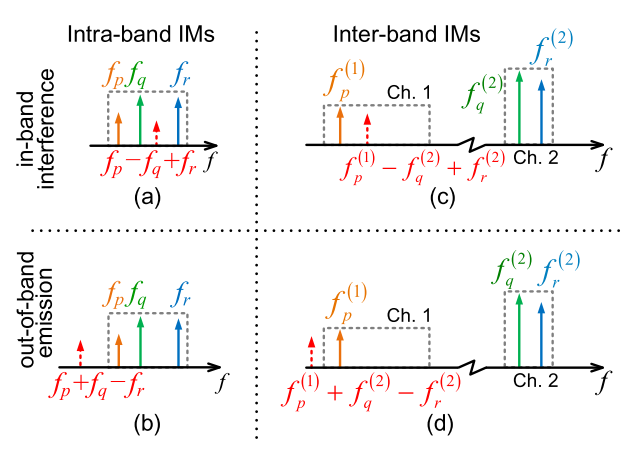
\includegraphics[width=0.65\textwidth]{IM}
        \caption{Operation principles of subcarrier IMs. (a) In-band interferences and (b) out-of-band emission induced by intra-band IMs. (c) In-band interferences and (d) out-of-band emission induced by inter-band IMs among one subcarrier of Ch. 1 and two subcarriers of Ch. 2.}
    \end{figure}
    
    
\end{frame}

\begin{frame}
    \frametitle{Nonlinear Subcarrier Intermodulations---Single and multiband \cite{Wang2017}}
    \begin{figure}[h]
        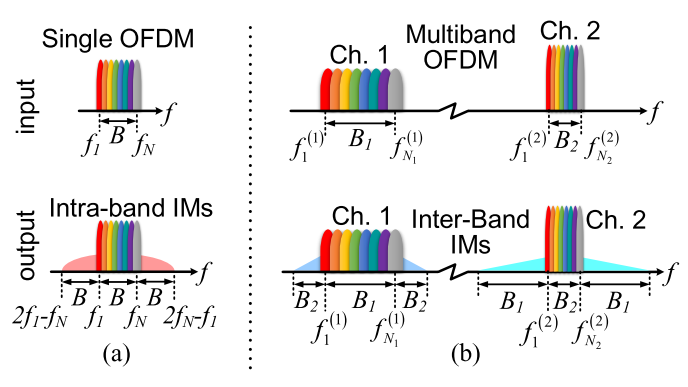
\includegraphics[width=0.9\textwidth]{single-and-multiband-IM.PNG}
        \caption{Nonlinear impairments of single-band and multiband OFDM signals. (a) Interference induced by intra-band IMs. (b) Interference induced by inter-band IMs.}
        
    \end{figure}
    
\end{frame}

\section{Mitigation}
\subsection{Conventional Digital Signal Processing}

\begin{frame}
    \frametitle{Linearization Technology Based on Digital Predistortion.}
    \begin{itemize}
        \item The dominant impairments in multi-carrier signals are subcarrier Intermodulations (IMs)
        \item Power amplifiers and electro-optic interface of optical modulators also major contributors of nonlinear channel response of analog MFH
        \item Power amplifiers are major sources of noise and MZM dominates the nonlinear impairments
        \item Linearization strategies can be used to mitigate this nonlinear impairments
        \item Predistortion technique is a great linearization technology 
        \item It is simple and low cost to implement, requiring only a block of predistorter befor the transmitter to pre-compensate the nonlinear channel response
        \item It can also be realized in the electrical domain without expensive optical equipment
    \end{itemize}
\end{frame}

\begin{frame}
    \frametitle{Digital Predistortion---How it works}
    \begin{itemize}
        \item Digital predistortion first transforms the input analog signals to digital domain
        \item After DSP, the processed signals are transformed back to analog domain by DAC
        \item The only constrain of digital predistortion is the processing speed, limited by the speed and power consumption of input/output ADC/DAC
        \item 
    \end{itemize}
\end{frame}

\begin{frame}
    \frametitle{Digital Predistortion---How it works (Block representation) \cite{Wang2017}}
    \begin{figure}
        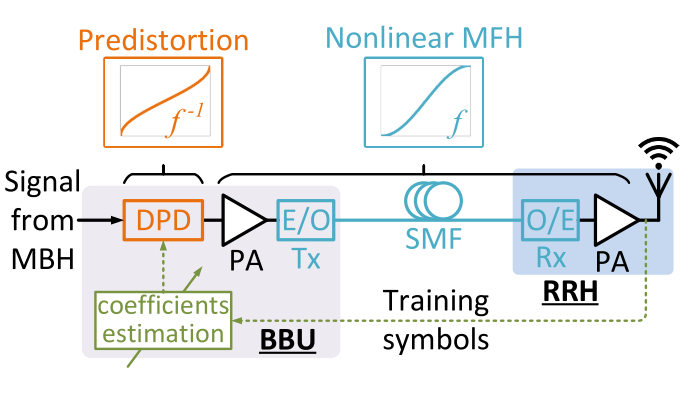
\includegraphics[width=\textwidth]{predistortion}
        \caption{Linearization based on digital predistortion for analog MFH.}
        \label{predistortion}
    \end{figure}
\end{frame}

\begin{frame}
    \frametitle{Digital Predistortion---How it works}
    \begin{itemize}
        \item The channel response and digital predistorter have two complimentary transfer functions, shown in inset of Fig. \ref{predistortion}
        \item The nonlinear response cancel each other and an overall linearized channel is obtained
        \item The transfer function of any bandwidth-limited nonlinear system can be modeled by polynomial with memory effect, as shown in equation \ref{memPolyModel}
        \item Memory effect is used to capture the inter-symbol interference (ISI)
        \item The memory depth equal the number of interfering symbols 
        \item Memory polynomial can model any nonlinear bandwidth-limited system, including amplifiers, modulators, and fiber dispersion and nonlinearities
    \end{itemize}
    
    
\end{frame}

\begin{frame}
    \frametitle{Digital Predistortion---Memory polynomial effect}
    \begin{figure}
        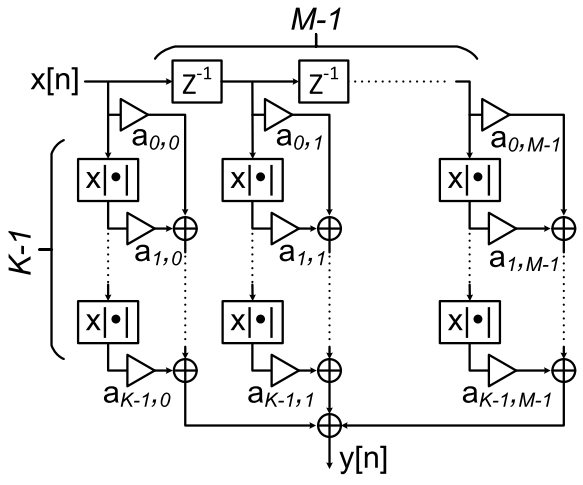
\includegraphics[width=0.7\textwidth]{memory-polynomial.PNG}
        \caption{Memory polynomial model of analog MFH channel with memory depth of M and nonlinearity order of K.}
        \label{memorypolynomial}
    \end{figure}
\end{frame}

\begin{frame}
    \frametitle{Digital Predistortion---Memory polynomial effect}
    \begin{equation}
         y\left[n\right] = \sum_{k=1}^{K}\sum_{m=1}^{M}a_{k,m}\cdot x\left[n-m+1\right]\cdot |x\left[n-m+1\right]|^{k-1} 
        \label{memPolyModel}
    \end{equation}
    \(y\left[n\right]\), the received signal---which is the distorted replica of 
    \(x\left[n\right]\)---is not only determined by the current input but also depends on few previous inputs \(x\left[n-m+1\right]\).
    \(M\) denotes the memory depth \(m=1,2,\ldots,M\).
    \(a_{k,m}\) is the polynomial coefficient of the \(k-th\) order term with memory depth \(m\).
    \(x\left[n\right]|x\left[n\right]|^{k-1}\) is the higher order terms, where \(k\) denotes the order of nonlinearity.

\end{frame}

\begin{frame}
    \frametitle{Digital Predistortion---Memory polynomial effect}
    \begin{itemize}
        \item In order to compensate for the nonlinear impairments in the channel, digital predistortion obtains the inverse function of (\ref{memPolyModel})
        \item This is simply achieved by reversing the roles of the input and output, and solving the inverse transfer function from output \(y\left[n\right]\) to input \(x\left[n\right]\), shown in (\ref{memPolyModelReverse})
        
    \end{itemize}
    \begin{equation}
        x\left[n\right] = \sum_{k=1}^{K}\sum_{m=1}^{M}d_{k,m}\cdot y\left[n-m+1\right]\cdot |y\left[n-m+1\right]|^{k-1} 
       \label{memPolyModelReverse}
    \end{equation}

    \begin{itemize}
        \item Training symbols were used in the experiment to estimate the inverse channel response and extract polynomial coefficients of \(d_{k,m}\)
        \item This can be done with matrix representation of the equations
    \end{itemize}


\end{frame}

\begin{frame}
    \frametitle{Digital Predistortion---Memory polynomial effect}
    \begin{figure}
        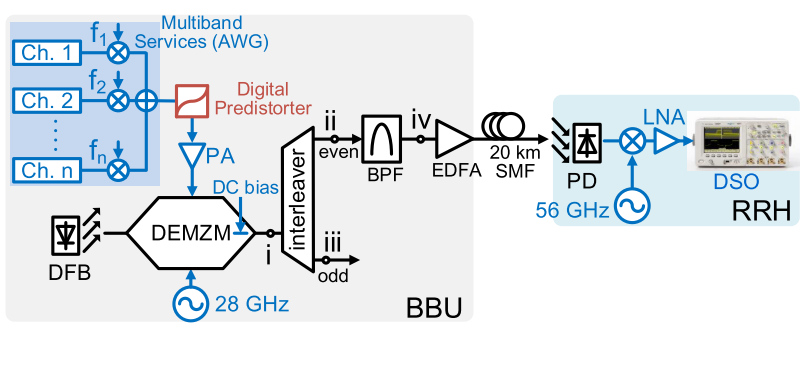
\includegraphics[width=\textwidth]{digitalPredistortionExperiment.PNG}
        \caption{Experimental setup of digital predistortion.}
    \end{figure}
\end{frame}


\subsection{Machine Learning Algorithms}
\begin{frame}
    \frametitle{Machine Learning-based nonlinear Mitigation}
    \begin{itemize}
        \item Nonlinear impairment mitigations based on Digital signal processing are expensive
        \item Due to their processing speed constrain, limited by the speed and power consumption of input/output ADC/DAC
        \item Mitigation of nonlinear impairments based on machine learning algorithms will be a much more cost effective alternative to mitigate nonlinearities
        \item 
    \end{itemize}
\end{frame}

\begin{frame}
    \frametitle{Review---Enhancement of UFMC based RoF System Using ANN Equalizer \cite{Liu2019}}
    \begin{itemize}
        \item Numerical simulation of UFMC waveform in RoF system equipped with ANN equalizer is performed by MATLAB and VPI
        \item The first UFMC symbol is used as the training sequence (\(1\%\) of total symbol lenght)
        \item Presents the constellation of the original received signals without dispersion compansation(DC) or equaliztion (EQ)
        \item Constellation points of signals equalized by ANN group more tightly and are condensed to the ideal points
        \item Presents the 
        \item This work proves that ANN equalizer is able to compensate for nonlinear impairments and achieves lower EVM than ZF equalizer
    \end{itemize}
\end{frame}

\begin{frame}
    \frametitle{Review---Enhancement of UFMC based RoF System Using ANN Equalizer \cite{Liu2019}}
    \begin{figure}
        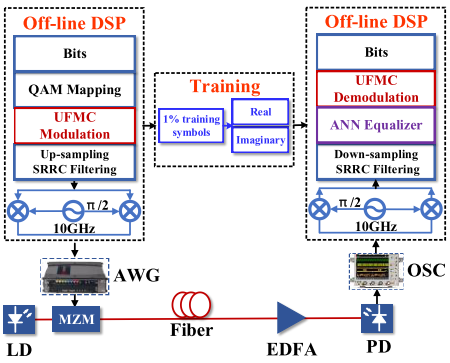
\includegraphics[width=0.7\textwidth]{ANNEqualizer.PNG}
        \caption{Structure of ANN equalizer based RoF system.}
    \end{figure}
\end{frame}

\begin{frame}
    \frametitle{Review---Enhancement of UFMC based RoF System Using ANN Equalizer \cite{Liu2019}}
    \begin{figure}
        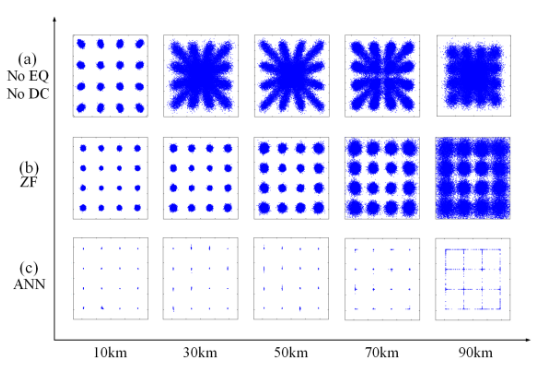
\includegraphics[width=0.8\textwidth]{ANNEqualizerConstellation.PNG}
        \caption{Constellation of UFMC waveforms for different fiber lengths (simulation)}
    \end{figure}
\end{frame}

\begin{frame}
    \frametitle{Review---Enhancement of UFMC based RoF System Using ANN Equalizer \cite{Liu2019}}
    \begin{figure}
        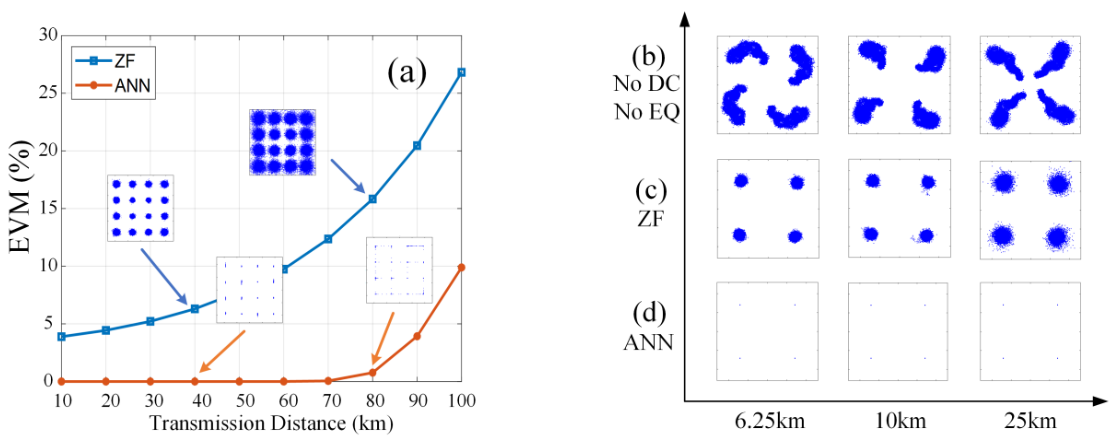
\includegraphics[width=\textwidth]{ANNEqualizerResult.PNG}
        \caption{(a) EVMs of UFMC waveforms for different transmission distances (simulation). (b)- (d) Constellations of UFMC waveforms with different equalizers for different transmission distances (experiment).}
    \end{figure}
\end{frame}

\begin{frame}
    \frametitle{Review---A Novel ANN Equalizer to mitigate Nonlinear Interference in Analog-RoF Nobile Fronthaul \cite{Liu2018a}}
    \begin{figure}
        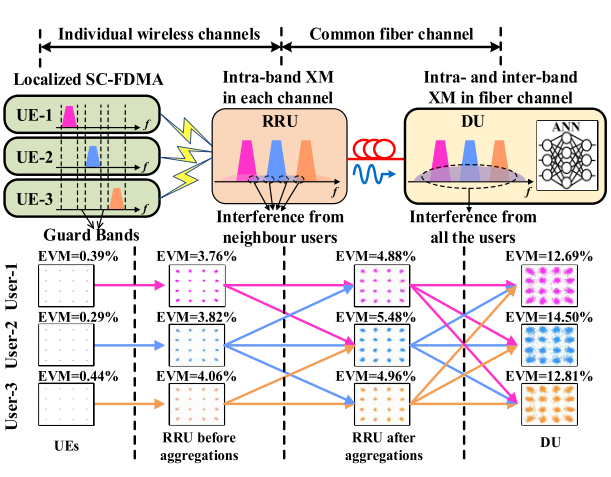
\includegraphics[width=0.6\textwidth]{novelANN.PNG}
        \caption{A-RoF-based fronthaul consisting of three individual wireless channels and one common fiber channel.}
    \end{figure}
\end{frame}

\begin{frame}
    \frametitle{Review---A Novel ANN Equalizer to mitigate Nonlinear Interference in Analog-RoF Nobile Fronthaul \cite{Liu2018a}}
    \begin{figure}
        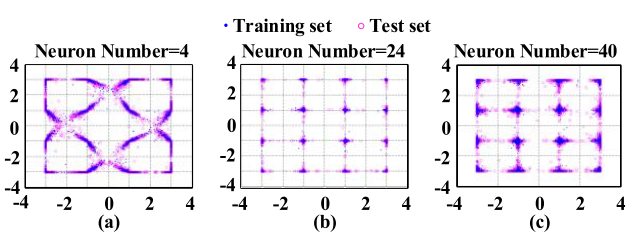
\includegraphics[width=\textwidth]{novelANNTraining.PNG}
        \caption{Constellations of the equalized signals when transmitting 4 users with (a) 4, (b) 24 and (c) 40 neurons in hidden layers.}
    \end{figure}
\end{frame}

\begin{frame}
    \frametitle{Review---A Novel ANN Equalizer to mitigate Nonlinear Interference in Analog-RoF Nobile Fronthaul \cite{Liu2018a}}
    \begin{figure}
        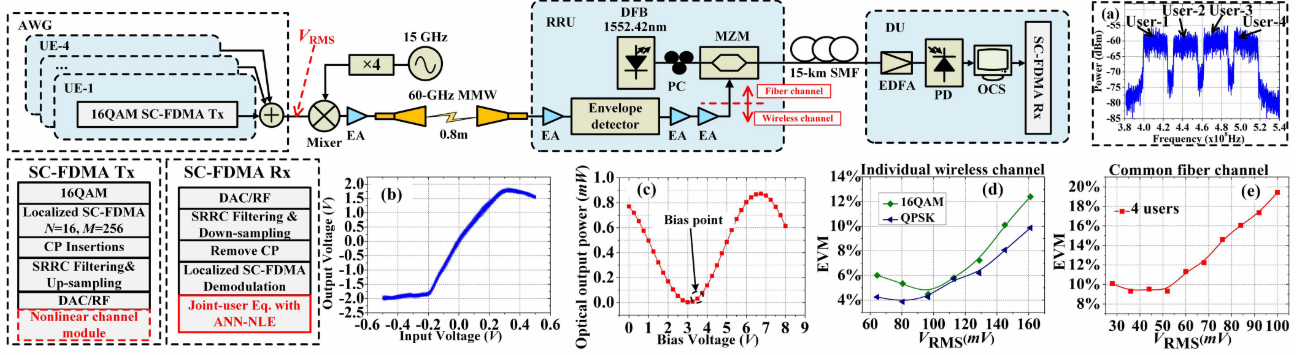
\includegraphics[width=\textwidth]{novelANNSetup.PNG}
        \caption{Experimental setup of the A-RoF-based MFH testbed that uses an ANN-NLE to co-equalize multiple users. 
        Inset (a) is the frequency spectrum of the 4 users at DU. (b) is the measured nonlinear transfer curve of the wireless channel. 
        (c) is the measured transfer curve of MZM, (d) and (e) are the EVMs of the received SC-FDMA signals as functions of VRMS at the 
        output of AWG when suffering from wireless channel nonlinearity and fiber nonlinearity.}
    \end{figure}
\end{frame}

\begin{frame}
    \frametitle{Review---A Novel ANN Equalizer to mitigate Nonlinear Interference in Analog-RoF Nobile Fronthaul \cite{Liu2018a}}
    \begin{figure}
            
        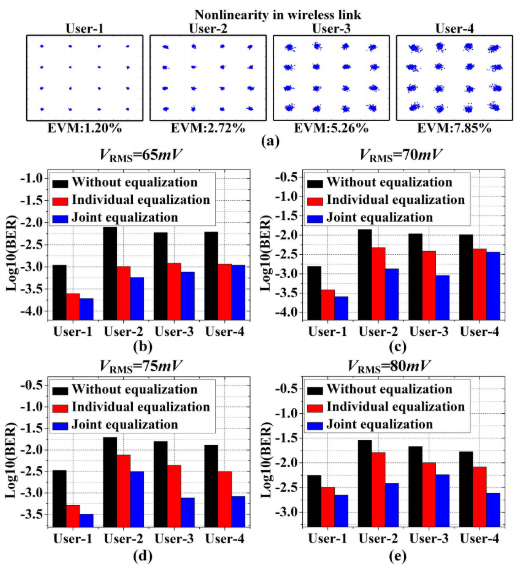
\includegraphics[width=0.6\textwidth]{novelANNResult.PNG}             
    \end{figure}
\end{frame}

\section{References}
\begin{frame}[t,allowframebreaks]
    \frametitle{References}
    \bibliographystyle{ieeetr}
    \bibliography{C:/Users/rajiy/Documents/MENDEL\string~1/library}
    
\end{frame}



    
\end{document}
